\subsection{Bubble \& eat - Fattorino}

\UC{Leggere la lista delle consegne da effettuare}{UC3.9}

\begin{figure}[H]
	\centering
	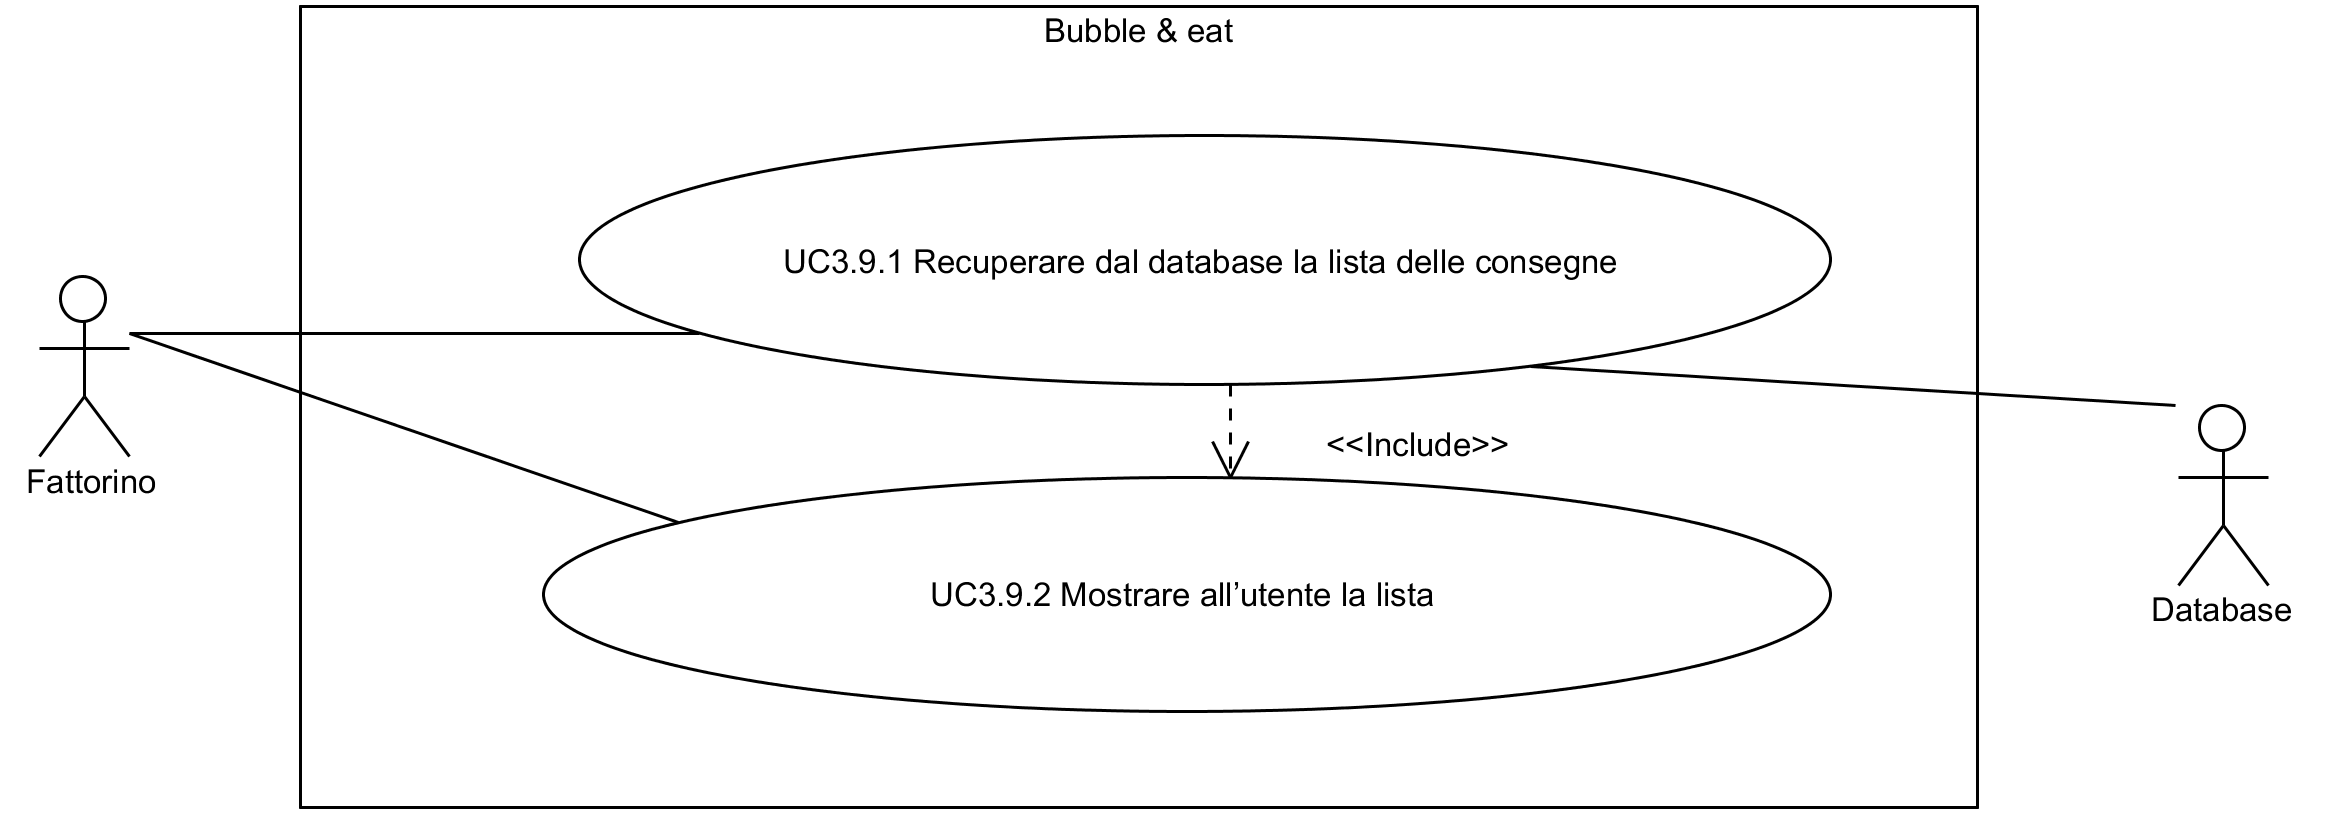
\includegraphics[width=15cm]{../../documenti/AnalisiDeiRequisiti/Diagrammi_img/uc3_9.png}
	\caption{\UCCaption{} Leggere la lista delle consegne da effettuare}
\end{figure}

\begin{itemize}
	\item \textbf{Attori:}
	\\Fattorino.
	\item \textbf{Scopo e descrizione:} 
	\\Lo scopo di questa funzionalità è permettere al Fattorino di consultare la lista delle consegne da effettuare.
	\item \textbf{Precondizioni:}
	\begin{itemize}
		\item Avere Rocket.Chat.
		\item Avere la bubble del ristorante selezionato.
		\item Avere accesso alla bubble con il ruolo Fattorino.
	\end{itemize}
	\item \textbf{Flusso principale degli eventi:}
	\begin{itemize}
		\item Il Fattorino seleziona la parte corrispondente della bubble.
		\item Viene recuperata dal database la lista delle consegne \ref{UC3.9.1}.
		\item Viene mostrata la lista all'utente \ref{UC3.9.2}.
	\end{itemize}
	\item \textbf{Post-condizione:}
	\\Il Fattorino è a conoscenza delle consegne da effettuare.
\end{itemize}

\UCF{Recuperare dal database la lista delle consegne}{UC3.9.1}

\begin{itemize}
	\item \textbf{Attori:}
	\\Fattorino.
	\item \textbf{Scopo e descrizione:} 
	\\Lo scopo di questa funzionalità è avere a disposizione nella memoria della bubble la lista delle consegne da effettuare.
	\item \textbf{Precondizioni:}
	\begin{itemize}
		\item Avere Rocket.Chat.
		\item Avere la bubble del ristorante selezionato.
		\item Avere accesso alla bubble con il ruolo Fattorino.
	\end{itemize}
	\item \textbf{Flusso principale degli eventi:}
	\\La bubble salva nella propria memoria la lista delle consegne.
	\item \textbf{Post-condizione:}
	\\Nella memoria della bubble è presente la lista delle consegne da effettuare.
\end{itemize}

\UCF{Mostrare al fattorino la lista}{UC3.9.2}

\begin{itemize}
	\item \textbf{Attori:}
	\\Fattorino.
	\item \textbf{Scopo e descrizione:} 
	\\Lo scopo di questa funzionalità è permettere al Fattorino di accedere e leggere la lista delle consegne da effettuare.
	\item \textbf{Precondizioni:}
	\begin{itemize}
		\item Avere Rocket.Chat.
		\item Avere la bubble del ristorante selezionato.
		\item Avere accesso alla bubble con il ruolo Fattorino.
	\end{itemize}
	\item \textbf{Flusso principale degli eventi:}
	\\La lista viene visualizzata.
	\item \textbf{Post-condizione:}
	\\La lista è visualizzata e il Fattorino è a conoscenza delle consegne da effettuare.
\end{itemize}

\UC{Selezionare la consegna da effettuare}{UC3.10}

\begin{figure}[H]
	\centering
	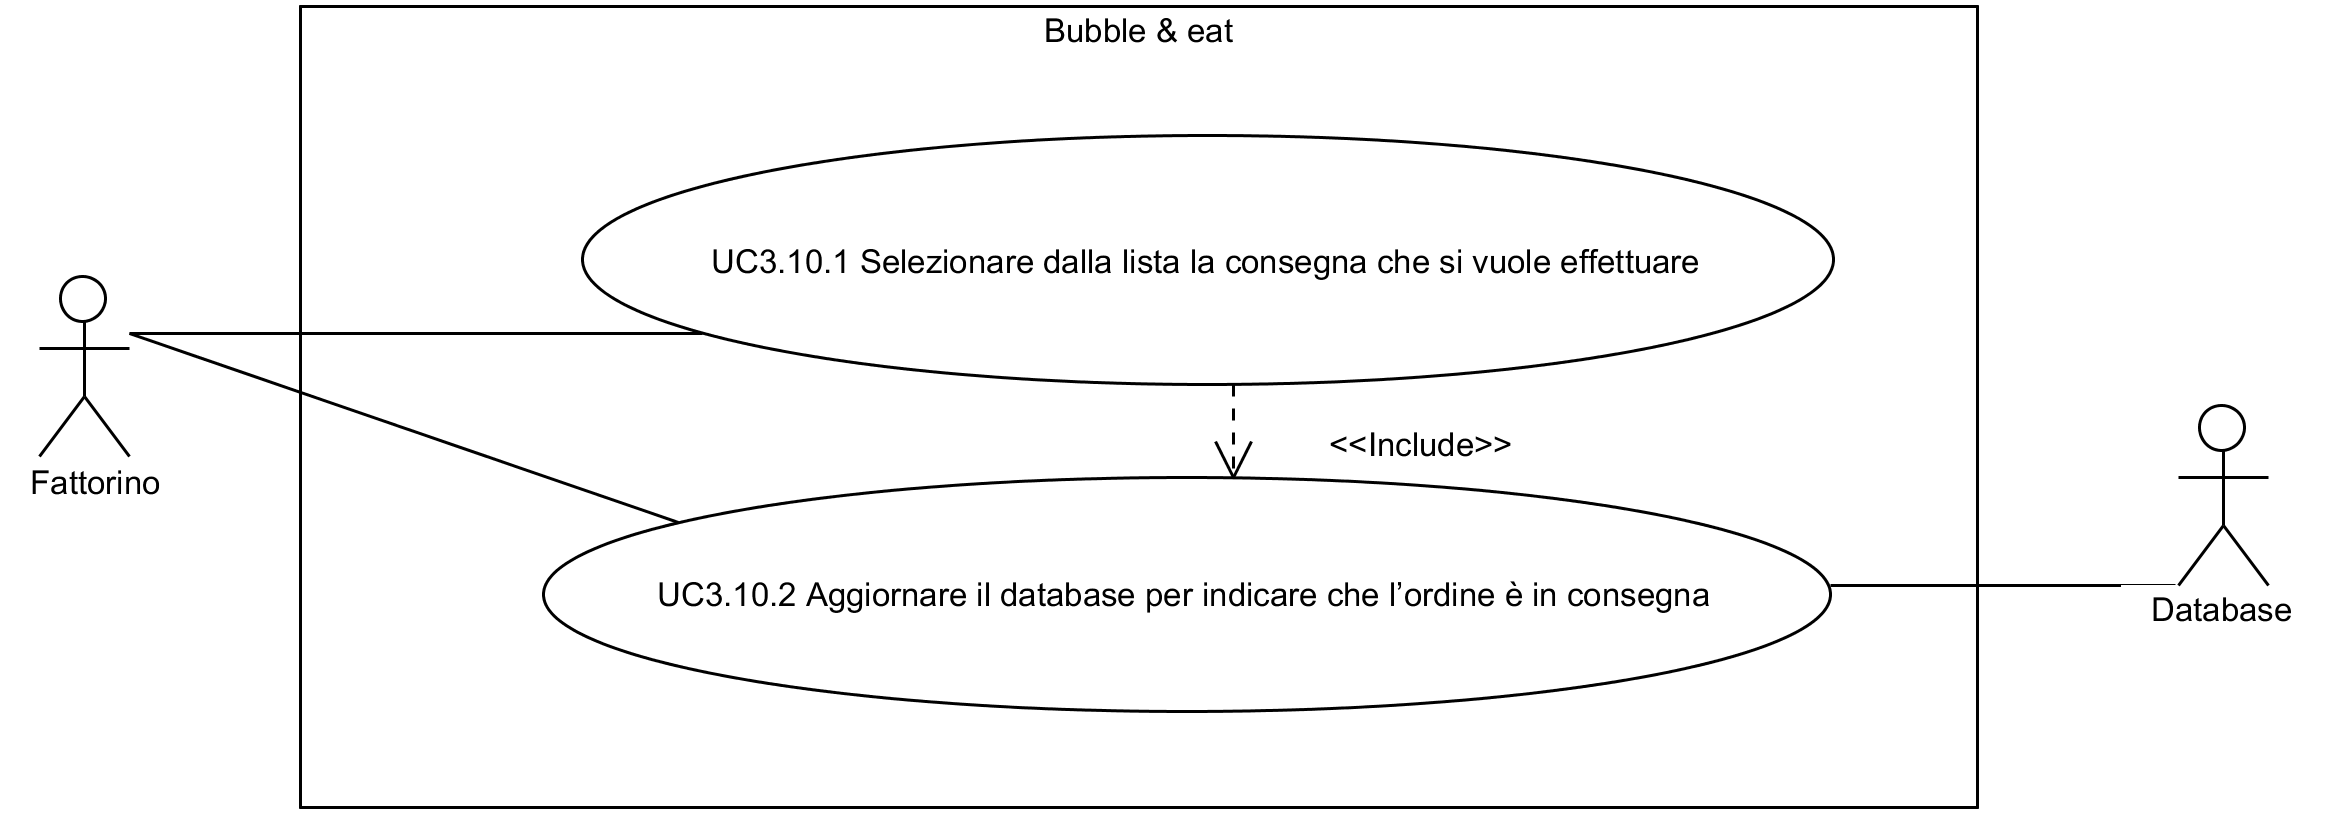
\includegraphics[width=15cm]{../../documenti/AnalisiDeiRequisiti/Diagrammi_img/uc3_10.png}
	\caption{\UCCaption{} Selezionare la consegna da effettuare}
\end{figure}

\begin{itemize}
	\item \textbf{Attori:}
	\\Fattorino.
	\item \textbf{Scopo e descrizione:} 
	\\Lo scopo di questa funzionalità è permettere al Fattorino di selezionare dalla lista delle consegne una da effettuare.
	\item \textbf{Precondizioni:}
	\begin{itemize}
		\item Avere Rocket.Chat.
		\item Avere la bubble del ristorante selezionato.
		\item Avere accesso alla bubble con il ruolo Fattorino.
		\item Visualizzare la lista delle consegne da effettuare \ref{UC3.9.2};
		\item Devono esistere consegne da effettuare.
	\end{itemize}
	\item \textbf{Flusso principale degli eventi:}
	\begin{itemize}
		\item Il Fattorino visualizza la lista delle consegne \ref{UC3.9}.
		\item Il Fattorino seleziona dalla lista quale consegna desidera effettuare \ref{UC3.10.1}.
		\item Il database viene aggiornato per indicare che l'ordine è in consegna \ref{UC3.10.2}.
	\end{itemize}
	\item \textbf{Post-condizione:}
	\\La lista delle consegne viene aggiornata e viene selezionata la consegna scelta.
\end{itemize}

\UCF{Selezionare dalla lista la consegna che si vuole effettuare}{UC3.10.1}

\begin{itemize}
	\item \textbf{Attori:}
	\\Fattorino.
	\item \textbf{Scopo e descrizione:} 
	\\Lo scopo di questa funzionalità è permettere al Fattorino di selezionare dalla lista delle consegne una da effettuare.
	\item \textbf{Precondizioni:}
	\begin{itemize}
		\item Avere Rocket.Chat.
		\item Avere la bubble del ristorante selezionato.
		\item Avere accesso alla bubble con il ruolo Fattorino.
		\item Devono esistere consegne da effettuare.
		\item La lista delle consegne da effettuare è visualizzata.
	\end{itemize}
	\item \textbf{Flusso principale degli eventi:}
	\\Il Fattorino seleziona dalla lista quale consegna desidera effettuare.
	\item \textbf{Post-condizione:}
	\\La consegna che il Fattorino vuole effettuare è selezionata.
\end{itemize}

\UCF{Aggiornare il database per indicare che l'ordine è in consegna}{UC3.10.2}

\begin{itemize}
	\item \textbf{Attori:}
	\\Fattorino.
	\item \textbf{Scopo e descrizione:} 
	\\Lo scopo di questa funzionalità è di aggiornare lo stato dell'ordine una volta che il Fattorino l'abbia preso in consegna.
	\item \textbf{Precondizioni:}
	\begin{itemize}
		\item Avere Rocket.Chat.
		\item Avere la bubble del ristorante selezionato.
		\item Avere accesso alla bubble con il ruolo Fattorino.
		\item Devono esistere consegne da effettuare.
		\item È stata selezionata una consegna da effettuare come indicato in \ref{UC3.10.1}.
	\end{itemize}
	\item \textbf{Flusso principale degli eventi:}
	\\Il Fattorino seleziona dalla lista quale consegna desidera effettuare.
	\item \textbf{Post-condizione:}
	\\L'ordine selezionato in \ref{UC3.10.1} è stato aggiornato nel database cambiandone lo stato in \virgolette{in consegna}.
\end{itemize}

\UC{Consegna effettuata}{UC3.11}

\begin{figure}[H]
	\centering
	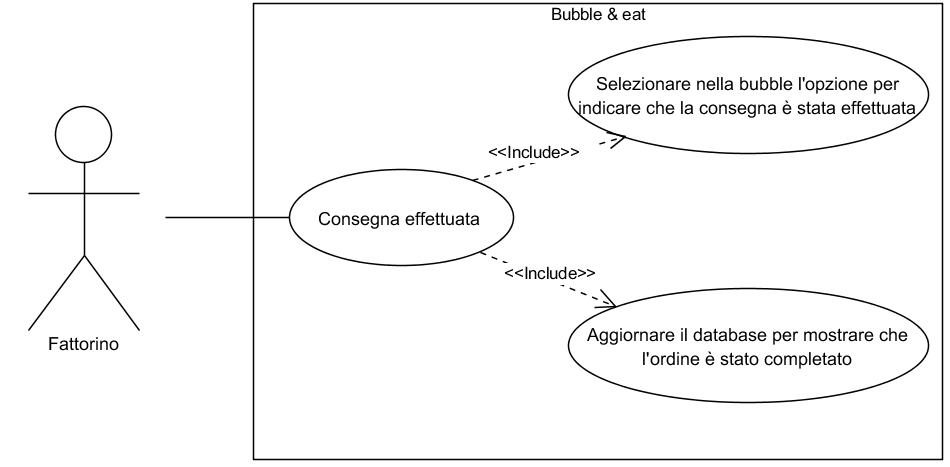
\includegraphics[width=15cm]{../../documenti/AnalisiDeiRequisiti/Diagrammi_img/uc3_11.png}
	\caption{\UCCaption{} Consegna effettuata}
\end{figure}

\begin{itemize}
	\item \textbf{Attori:}
	\\Fattorino.
	\item \textbf{Scopo e descrizione:} 
	\\Lo scopo di questa funzionalità è permettere al Fattorino di confermare l'effettuazione della consegna.
	\item \textbf{Precondizioni:}
	\begin{itemize}
		\item Avere Rocket.Chat.
		\item Avere la bubble del ristorante selezionato.
		\item Avere accesso alla bubble con il ruolo Fattorino.
		\item Deve essere stata selezionata una consegna dalla lista.
	\end{itemize}
	\item \textbf{Flusso principale degli eventi:}
	\begin{itemize}
		\item Il Fattorino indica che la consegna è stata effettuata \ref{UC3.11.1}.
		\item Il database viene aggiornato \ref{UC3.11.2}.
	\end{itemize}
	\item \textbf{Post-condizione:}
	\\La lista delle consegne viene aggiornata e viene eliminata la consegna effettuata.
\end{itemize}

\UCF{Selezionare nella bubble l'opzione per indicare che la consegna è stata effettuata}{UC3.11.1}

\begin{itemize}
	\item \textbf{Attori:}
	\\Fattorino.
	\item \textbf{Scopo e descrizione:} 
	\\Lo scopo di questa funzionalità è di notificare l'avvenuta consegna della pietanza all'indirizzo inviato dall'utente.
	\item \textbf{Precondizioni:}
	\begin{itemize}
		\item Avere Rocket.Chat.
		\item Avere la bubble del ristorante selezionato.
		\item Avere accesso alla bubble con il ruolo Fattorino.
		\item Deve essere stata selezionata una consegna dalla lista.
		\item La consegna deve essere stata effettuata.
	\end{itemize}
	\item \textbf{Flusso principale degli eventi:}
	\\Il Fattorino indica quando la consegna viene portata a termine.
	\item \textbf{Post-condizione:}
	\\Nella bubble del Fattorino è salvato lo stato che la consegna è stata effettuata con successo.
\end{itemize}

\UCF{Aggiornare il database per mostrare che l'ordine è stato completato}{UC3.11.2}

\begin{itemize}
	\item \textbf{Attori:}
	\\Fattorino.
	\item \textbf{Scopo e descrizione:} 
	\\Lo scopo di questa funzionalità è aggiornare il database quando un Fattorino conferma l'effettuazione della consegna.
	\item \textbf{Precondizioni:}
	\begin{itemize}
		\item Avere Rocket.Chat.
		\item Avere la bubble del ristorante selezionato.
		\item Avere accesso alla bubble con il ruolo Fattorino.
		\item Deve essere stata selezionata una consegna dalla lista per essere segnata come completata.
	\end{itemize}
	\item \textbf{Flusso principale degli eventi:}
	\\Vengono aggiornati i dati nel database quando una consegna viene confermata.
	\item \textbf{Post-condizione:}
	\\I dati nel database sono aggiornati.
\end{itemize}